\chapter{Previous Research}
The choice of programming languages was based on a study that ranked different programming languages by their energy efficiency. The study pitted ten programming languages against each other, using “rigorous and strict solutions to 10 well-defined programming problems, expressed in (up to) 27 programming languages, from the well known Computer Language Benchmark Game repository.” \cite{PEREIRA2021102609} Results of the study showed that C++, C and Rust were the most energy and time efficient languages, with Pascal and Go scoring higher on memory efficiency, as seen in figure 4.1. Python consistently scored in second to last place for energy and time efficiency and in 12th place (out of 27 languages) for memory efficiency.
C++ was chosen based on the libraries available for the chosen aim of the program and because it was one of the best performing languages in this study.
Python was chosen because it was one of the three worst-performing languages in the study.

\begin{figure}[htbp]
	\centering
	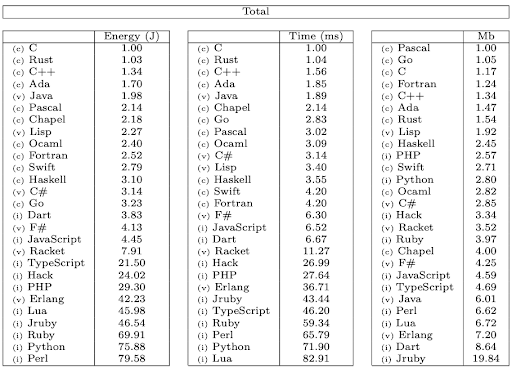
\includegraphics[scale=0.70]{previous-research-languages.png}
	\caption{Normalised global results for Energy, Time, and Memory \cite[p.16]{PEREIRA2021102609}}
	\label{figure:previous-research-languages}
\end{figure}
